\chapter{Spatial Domain: \refmod}
\label{ch:ref-mod}

It was Xenakis' goal for the curved surfaces of the Philips Pavilion
to reduce the sonic contribution of sound reflections as much as
possible.\cite{philips1958} He knew that reflections and the resulting
comb filtering could impair intelligibility and localization of music
and sounds.  The pavilion was to have hundreds of loudspeakers, and an
elaborate custom sequencer electronically selected which speakers
Edgard Var\`{e}se's music played from. However, large concave surfaces
like the ones on the inside of the pavilion can have a focussing
effect on acoustic reflections,\cite{Vercammen2008} which may result
in severe filtering and phase cancellations. There is evidence that
carefully constructed curved surfaces such as stage shells can be
effective for performers of acoustic music.\cite{DAntonio1991}
In the context of loudspeaker playback, the advantages of
curved surfaces over flat (non-parallel) surfaces are ambiguous at
best.\cite{Cox2006} When we hear an acoustic sound reflection off a
concave surface, the sound can arrive at our ears in two possible
states:
\begin{enumerate}
\item The path of the sound from the source to the reflecting surface
  to our ears is equidistant for each point on the reflecting
  surface. Ignoring any direct sound, the reflection arrives in-phase,
  and the surface acts as acoustic amplifier of the reflection.
\item The path of the sound from the source to the reflecting surface
  to our ears is slightly different for each point on the surface. All
  the reflections arrive out of phase with each other.
\end{enumerate}
Parabolic microphones\sidenote[][-32mm]{Parabolic microphones use a
  specially designed parabolic reflector that focuses sound arriving
  from one direction on the microphone capsule. Handheld models are
  commonly used in birdsong recording, and on the sidelines of
  football games. They typically have a diameter of two feet or less,
  and can capture sound up to 500 feet away. Due to the size of the
  reflector, commercial parabolic microphones cannot capture sounds
  below approximately 1kHz.}\cite{Davis1989}, and acoustic whispering
chambers\sidenote{A room built such that the walls are angled to
  direct sound from one corner to another. If two people stand in the
  correct spaces in a whispering chamber, they can clearly hear each
  other whispering even though they may be at opposite ends of the
  room.} fall into the first category. Both use surfaces that are
angled to reflect all sound emanating from one direction to converge
at a certain point. If a concave surface reflecting surfaces is not
carefully designed to focus sounds \textit{in phase} it is much more
likely that the sounds will arrive out of phase. The curves of the
Philips Pavilion probably created an \emph{unusual} acoustic space,
rather than a good space for critical listening. However, this may
have been advantageous to the project: Part of the spectacle was
seeing, hearing, and experiencing something completely unprecedented
and unlike anything else.

\section{Composing with Space}
\label{sec:composing-with-space}
If Xenakis had been able to model the reflections and compose them
directly into the piece, what would the tools be like? How can we make
the difference between in phase reflections and out of phase
reflections intuitive?  It we had tools available to compose with
acoustic reflections, how could we use controlled filtering
creatively, and what kind of music, and architectural spaces would we
make? The Xenakis inspired \refmod is an abstract software tool for
experimenting with architectural acoustic lenses. It is intended more
as an experiment for architectural or musical brainstorming than as a
simulation for analysis of sound propagation. For example:
\begin{enumerate}
\item It illustrates sound projection in only two dimensions.
\item It is frequency independent. Real sufaces reflect only
  wavelengths much smaller than the size of the
  reflector.\cite{Zhixin2005} 
\item Diffraction is ignored. 
\item Acoustic sounds waves of higher frequencies propagate more
  directionally than lower frequencies. This property is ignored.
% \item The acoustic reflections from, and acoustic diffraction around a
%   real object are dependent on the materials and obstacles behind
%   or adjacent the reflecting surface.\cite{Howard2006} This effect is
%   also not taken modeled by the \refmod.
\end{enumerate}

\section{Implementation}
\label{sec:refmod-implementation}
The \refmod was implemented as a web app using the HTML5
Paper.js\sidenote{\url{http://paperjs.org/}} vector graphics
library. Try it out online at\\
\noindent \url{http://web.media.mit.edu/~holbrow/mas/reflections/}

\section{\refmod Architectural Example}
\label{sec:refmod-user-interf}
Assume we are creating the floor plan for a new architectural space
and accompanying electronic music performance. We want to use acoustic
reflections to create certain sounds at certain locations in the
performance space. We can use the this tool to prototype potential
layouts. The curved black line in the user interface
(figure~\ref{fig:refmod-simple}) represents a reflective surface. The
black dot with emanating red lines represents a sound source, and the
sound propagation. Click and drag on any black dot to move the
object. Black dots connected by grey lines are handles that
re-orient (instead of move) objects. On reflection surfaces, the handles
adjust the angle and shape of the surface curve. Handles connected to
sound sources adjust the angle and length of the sound beams. 
\begin{figure}[]
% http://web.media.mit.edu/~holbrow/mas/reflections/?q=%7B%22mirrors%22%3A%5B%5B%22Path%22%2C%7B%22applyMatrix%22%3Atrue%2C%22segments%22%3A%5B%5B%5B330%2C60%5D%2C%5B0%2C0%5D%2C%5B-239%2C185%5D%5D%2C%5B319%2C424%5D%5D%2C%22strokeColor%22%3A%5B0%2C0%2C0%5D%2C%22strokeWidth%22%3A2%7D%5D%2C%5B%22Path%22%2C%7B%22applyMatrix%22%3Atrue%2C%22segments%22%3A%5B%5B%5B1035%2C436%5D%2C%5B0%2C0%5D%2C%5B-135%2C113%5D%5D%2C%5B1123%2C534%5D%5D%2C%22strokeColor%22%3A%5B0%2C0%2C0%5D%2C%22strokeWidth%22%3A2%7D%5D%5D%2C%22sounds%22%3A%5B%5B%22Path%22%2C%7B%22applyMatrix%22%3Atrue%2C%22segments%22%3A%5B%5B1047%2C123%5D%2C%5B1048%2C145%5D%5D%2C%22strokeColor%22%3A%5B0.6%2C0.6%2C0.6902%5D%7D%5D%2C%5B%22Path%22%2C%7B%22applyMatrix%22%3Atrue%2C%22segments%22%3A%5B%5B411%2C176%5D%2C%5B480%2C136%5D%5D%2C%22strokeColor%22%3A%5B0.6%2C0.6%2C0.6902%5D%7D%5D%5D%7D
  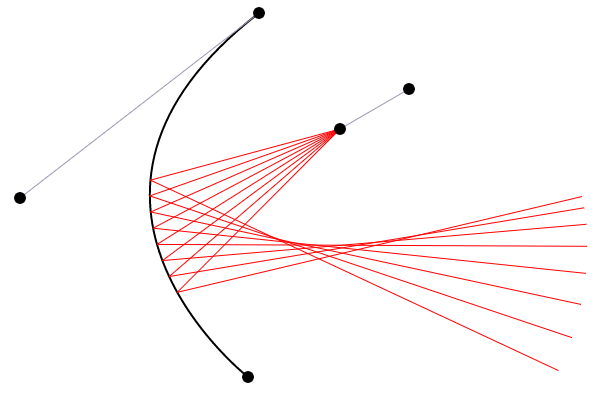
\includegraphics[width=\linewidth]{refmod/1.png}
  \caption[]{\refmod user interface.}
  \label{fig:refmod-simple}
\end{figure}
Each red line emanating from a sound source is the same length, no
matter how many times it has been reflected. If it is possible to
adjust the length of the red lines such that each one ends at the same
spot, it shows that reflections will arrive at that spot in
phase. Figures~\ref{fig:refmod-bad-focus}
and~\ref{fig:refmod-good-focus} show how we can adjust the curve of a
surface to focus reflections on a point.

\section{\refmod Musical Example}
\label{sec:refm-music-example}
The red emanating lines can also be thought of as stochastic pitch
swarms, similar to those Xenakis wrote for Metastasis in 1954
(figure~\ref{fig:metastasis}).
\TODO{Add Musical Example}

\begin{figure}[]
% http://web.media.mit.edu/~holbrow/mas/reflections/?q=%7B%22mirrors%22%3A%5B%5B%22Path%22%2C%7B%22applyMatrix%22%3Atrue%2C%22segments%22%3A%5B%5B%5B513%2C318%5D%2C%5B0%2C0%5D%2C%5B-218%2C117%5D%5D%2C%5B192%2C241%5D%5D%2C%22strokeColor%22%3A%5B0%2C0%2C0%5D%2C%22strokeWidth%22%3A2%7D%5D%2C%5B%22Path%22%2C%7B%22applyMatrix%22%3Atrue%2C%22segments%22%3A%5B%5B%5B1035%2C436%5D%2C%5B0%2C0%5D%2C%5B-135%2C113%5D%5D%2C%5B1123%2C534%5D%5D%2C%22strokeColor%22%3A%5B0%2C0%2C0%5D%2C%22strokeWidth%22%3A2%7D%5D%5D%2C%22sounds%22%3A%5B%5B%22Path%22%2C%7B%22applyMatrix%22%3Atrue%2C%22segments%22%3A%5B%5B1047%2C123%5D%2C%5B1048%2C145%5D%5D%2C%22strokeColor%22%3A%5B0.6%2C0.6%2C0.6902%5D%7D%5D%2C%5B%22Path%22%2C%7B%22applyMatrix%22%3Atrue%2C%22segments%22%3A%5B%5B220%2C202%5D%2C%5B177%2C150%5D%5D%2C%22strokeColor%22%3A%5B0.6%2C0.6%2C0.6902%5D%7D%5D%5D%7D
  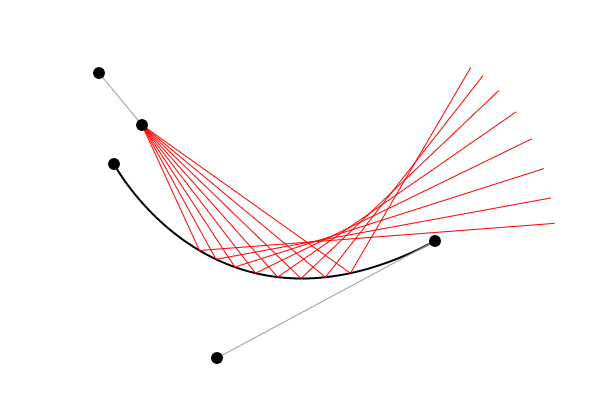
\includegraphics[width=\linewidth]{refmod/out-of-focus.png}
  \caption[]{Reflections from a $30\degree$ loudspeaker arriving out of phase.}
  \label{fig:refmod-bad-focus}
\end{figure}

\begin{figure}[]
%http://web.media.mit.edu/~holbrow/mas/reflections/?q=%7B%22mirrors%22%3A%5B%5B%22Path%22%2C%7B%22applyMatrix%22%3Atrue%2C%22segments%22%3A%5B%5B%5B525%2C318%5D%2C%5B0%2C0%5D%2C%5B-251%2C68%5D%5D%2C%5B180%2C242%5D%5D%2C%22strokeColor%22%3A%5B0%2C0%2C0%5D%2C%22strokeWidth%22%3A2%7D%5D%2C%5B%22Path%22%2C%7B%22applyMatrix%22%3Atrue%2C%22segments%22%3A%5B%5B%5B1035%2C436%5D%2C%5B0%2C0%5D%2C%5B-135%2C113%5D%5D%2C%5B1123%2C534%5D%5D%2C%22strokeColor%22%3A%5B0%2C0%2C0%5D%2C%22strokeWidth%22%3A2%7D%5D%5D%2C%22sounds%22%3A%5B%5B%22Path%22%2C%7B%22applyMatrix%22%3Atrue%2C%22segments%22%3A%5B%5B1047%2C123%5D%2C%5B1048%2C145%5D%5D%2C%22strokeColor%22%3A%5B0.6%2C0.6%2C0.6902%5D%7D%5D%2C%5B%22Path%22%2C%7B%22applyMatrix%22%3Atrue%2C%22segments%22%3A%5B%5B220%2C202%5D%2C%5B179%2C145%5D%5D%2C%22strokeColor%22%3A%5B0.6%2C0.6%2C0.6902%5D%7D%5D%5D%7D
  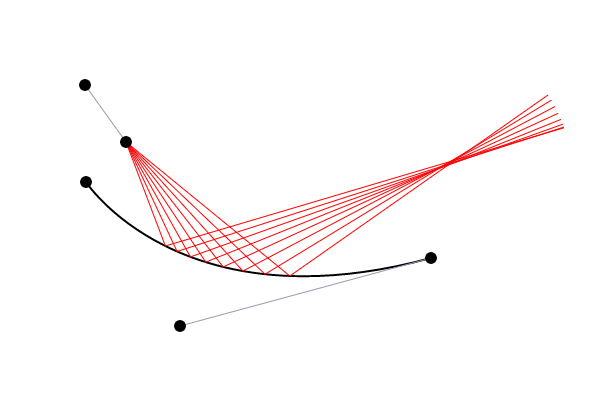
\includegraphics[width=\linewidth]{refmod/in-focus.png}
  \caption[]{By adjusting the curvature of the reflective surface, we
    can focus the audio reflections.}
  \label{fig:refmod-good-focus}
\end{figure}


\begin{figure*}[]
  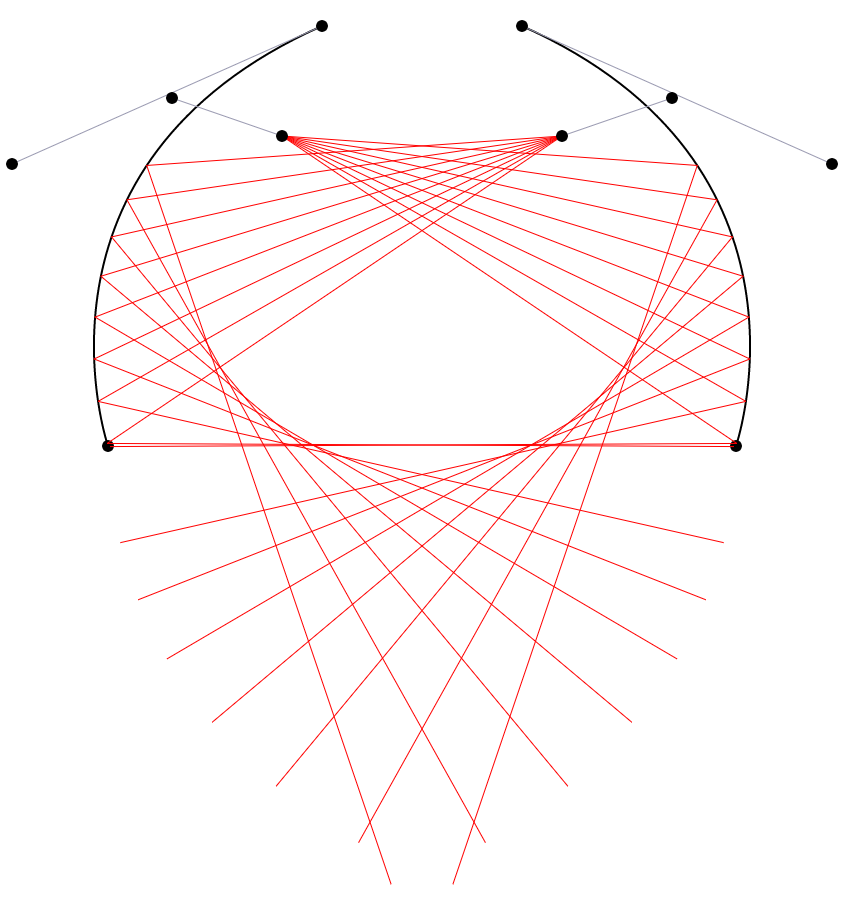
\includegraphics[width=\linewidth]{refmod/refmod.png}
  \caption[]{\refmod user interface.}
  \label{fig:refmod-full}
\end{figure*}


%%% Local Variables:
%%% mode: latex
%%% TeX-master: "CharlesHolbrow_MAS_Thesis"
%%% End:
